% Practice Test 07 — Florida Edition
% Questions: 30 (18 MC + 12 SA)
% Generated by scripts/generate_practice_tests.py

\begin{practiceQuestion}{1-3-q23}{sa}
\begin{questionText}
Two quantities are proportional with $k = 7$. If $y = 56$, what is $x$?
\end{questionText}
\correctAnswer{$x = 8$}
\explanation{$y = kx$ so $56 = 7x$, giving $x = 56 \div 7 = 8$.}
\end{practiceQuestion}

\begin{practiceQuestion}{1-6-q09}{mc}
\begin{questionText}
Which strategy is NOT a proportional reasoning tool?
\end{questionText}
\choiceA{Find the unit rate and multiply}
\choiceB{Set up a proportion and cross-multiply}
\choiceC{Use $y = kx$}
\choiceD{Add a fixed amount to each value}
\correctAnswer{D}
\explanation{Adding a fixed amount is an additive strategy, not proportional. Proportional strategies use multiplication and division.}
\end{practiceQuestion}

\begin{practiceQuestion}{2-1-q29}{gsa}
\begin{questionText}
Look at the $10 \times 10$ grid below. What percent of the grid is \textbf{not} shaded?

\begin{center}
\begin{tikzpicture}[scale=0.35]
  \foreach \x in {0,...,9} {
    \foreach \y in {0,...,9} {
      \draw[gray!50] (\x,\y) rectangle (\x+1,\y+1);
    }
  }
  % Shade 72 squares (rows 0-6 full = 70, plus 2 in row 7)
  \foreach \x in {0,...,9} {
    \foreach \y in {0,...,6} {
      \fill[funOrange!40] (\x,\y) rectangle (\x+1,\y+1);
      \draw[gray!50] (\x,\y) rectangle (\x+1,\y+1);
    }
  }
  \foreach \x in {0,...,1} {
    \fill[funOrange!40] (\x,7) rectangle (\x+1,8);
    \draw[gray!50] (\x,7) rectangle (\x+1,8);
  }
\end{tikzpicture}
\end{center}
\end{questionText}
\correctAnswer{$28\%$}
\explanation{Shaded squares: $7$ full rows of $10 = 70$, plus $2 = 72$. Unshaded: $100 - 72 = 28$. So $28\%$ is not shaded.}
\end{practiceQuestion}

\begin{practiceQuestion}{2-2-q27}{gmc}
\begin{questionText}
The bar model below represents a whole amount. Use the model to find what percent the shaded part is of the whole.

\begin{center}
\begin{tikzpicture}[scale=0.65]
  % Whole bar divided into 8 equal parts, 3 shaded
  \foreach \i in {0,...,7} {
    \draw[thick] (\i*1,0) rectangle (\i*1+1,0.8);
  }
  \fill[funBlue!40] (0,0) rectangle (1,0.8);
  \fill[funBlue!40] (1,0) rectangle (2,0.8);
  \fill[funBlue!40] (2,0) rectangle (3,0.8);
  \foreach \i in {0,...,7} {
    \draw[thick] (\i*1,0) rectangle (\i*1+1,0.8);
  }
  \draw[thick,<->] (0,-0.4) -- (3,-0.4) node[midway,below,font=\small] {$45$};
  \draw[thick,<->] (0,-1.1) -- (8,-1.1) node[midway,below,font=\small] {Whole $= {?}$};
  \node[above,font=\small] at (1.5,0.8) {Shaded};
\end{tikzpicture}
\end{center}

If each section has the same value and there are $8$ equal sections total, what percent is shaded?
\end{questionText}
\choiceA{$25\%$}
\choiceB{$33\%$}
\choiceC{$37.5\%$}
\choiceD{$45\%$}
\correctAnswer{C}
\explanation{$3$ out of $8$ sections are shaded. $\frac{3}{8} = \frac{p}{100}$ → $p = 37.5\%$.}
\end{practiceQuestion}

\begin{practiceQuestion}{2-6-q19}{sa}
\begin{questionText}
Find the simple interest: $P = \$3{,}500$, $r = 4\%$, $t = 2$ years.
\end{questionText}
\correctAnswer{$\$280$}
\explanation{$I = 3{,}500 \times 0.04 \times 2 = \$280$.}
\end{practiceQuestion}

\begin{practiceQuestion}{2-7-q21}{sa}
\begin{questionText}
A baker expected to make $80$ cookies from a recipe but made $72$. What is the percent error (rounded to the nearest tenth)?
\end{questionText}
\correctAnswer{$\approx 11.1\%$}
\explanation{$\frac{|80 - 72|}{72} \times 100 = \frac{8}{72} \times 100 \approx 11.1\%$.}
\end{practiceQuestion}

\begin{practiceQuestion}{3-2-q12}{mc}
\begin{questionText}
What is $(-7) + 7 + (-3)$?
\end{questionText}
\choiceA{$-3$}
\choiceB{$3$}
\choiceC{$-17$}
\choiceD{$17$}
\correctAnswer{A}
\explanation{$(-7) + 7 = 0$ (opposites cancel). Then $0 + (-3) = -3$.}
\end{practiceQuestion}

\begin{practiceQuestion}{3-3-q04}{mc}
\begin{questionText}
What is $(-4) - (-4)$?
\end{questionText}
\choiceA{$-8$}
\choiceB{$8$}
\choiceC{$0$}
\choiceD{$-16$}
\correctAnswer{C}
\explanation{$(-4) - (-4) = (-4) + 4 = 0$. Any number minus itself equals $0$.}
\end{practiceQuestion}

\begin{practiceQuestion}{4-4-q16}{mc}
\begin{questionText}
What is the GCF of $9x$, $12x$, and $15x$?
\end{questionText}
\choiceA{$x$}
\choiceB{$3$}
\choiceC{$3x$}
\choiceD{$9x$}
\correctAnswer{C}
\explanation{GCF of $9$, $12$, and $15$ is $3$. All terms share $x$. So the GCF is $3x$.}
\end{practiceQuestion}

\begin{practiceQuestion}{4-5-q08}{mc}
\begin{questionText}
Simplify $(-4x + 6) + (7x - 9)$.
\end{questionText}
\choiceA{$3x - 3$}
\choiceB{$-11x - 3$}
\choiceC{$3x + 3$}
\choiceD{$-3x + 15$}
\correctAnswer{A}
\explanation{Combine: $(-4x + 7x) + (6 - 9) = 3x - 3$.}
\end{practiceQuestion}

\begin{practiceQuestion}{5-3-q13}{mc}
\begin{questionText}
Solve $-5(x + 1) = -30$.
\end{questionText}
\choiceA{$x = 5$}
\choiceB{$x = -7$}
\choiceC{$x = 7$}
\choiceD{$x = -5$}
\correctAnswer{A}
\explanation{Divide by $-5$: $x + 1 = 6$. Subtract $1$: $x = 5$. Check: $-5(5 + 1) = -5(6) = -30$ \checkmark.}
\end{practiceQuestion}

\begin{practiceQuestion}{5-4-q17}{mc}
\begin{questionText}
Solve $\dfrac{x}{5} + \dfrac{3}{10} = \dfrac{7}{10}$.
\end{questionText}
\choiceA{$x = 4$}
\choiceB{$x = 5$}
\choiceC{$x = 1$}
\choiceD{$x = 2$}
\correctAnswer{D}
\explanation{Multiply every term by $10$: $2x + 3 = 7$. Subtract $3$: $2x = 4$. Divide by $2$: $x = 2$. Check: $\frac{2}{5} + \frac{3}{10} = \frac{4}{10} + \frac{3}{10} = \frac{7}{10}$ \checkmark.}
\end{practiceQuestion}

\begin{practiceQuestion}{5-5-q20}{sa}
\begin{questionText}
Solve $-5n + 10 \leq -15$.
\end{questionText}
\correctAnswer{$n \geq 5$}
\explanation{Subtract $10$: $-5n \leq -25$. Divide by $-5$ and flip: $n \geq 5$.}
\end{practiceQuestion}

\begin{practiceQuestion}{5-6-q26}{gmc}
\begin{questionText}
Which inequality matches the graph below?

\begin{center}
\begin{tikzpicture}[scale=0.7]
  \draw[thick,->] (-5,0) -- (5,0);
  \foreach \x in {-4,...,4} \draw (\x,0.15) -- (\x,-0.15) node[below] {$\x$};
  \draw[thick,funBlue,<-] (-5,0) -- (1,0);
  \fill[funBlue] (1,0) circle (4pt);
\end{tikzpicture}
\end{center}
\end{questionText}
\choiceA{$x \leq 1$}
\choiceB{$x < 1$}
\choiceC{$x \geq 1$}
\choiceD{$x > 1$}
\correctAnswer{A}
\explanation{Closed circle at $1$ with shading to the left means $x \leq 1$.}
\end{practiceQuestion}

\begin{practiceQuestion}{6-2-q29}{gsa}
\begin{questionText}
The rectangle below is drawn at scale $1$ cm $= 8$ m. Redraw it at scale $1$ cm $= 4$ m. What are the new dimensions, and what is the new drawing's area?

\begin{center}
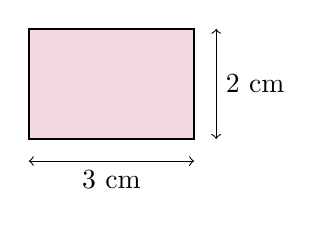
\begin{tikzpicture}[scale=0.7]
  \draw[thick,fill=purple!15] (0,0) rectangle (3,2);
  \draw[<->] (0,-0.4) -- (3,-0.4);
  \node[below] at (1.5,-0.4) {$3$ cm};
  \draw[<->] (3.4,0) -- (3.4,2);
  \node[right] at (3.4,1) {$2$ cm};
\end{tikzpicture}
\end{center}
\end{questionText}
\correctAnswer{$6$ cm by $4$ cm; area $= 24$ cm$^2$}
\explanation{Scale ratio: $\frac{8}{4} = 2$. New dimensions: $3 \times 2 = 6$ cm and $2 \times 2 = 4$ cm. Area: $6 \times 4 = 24$ cm$^2$.}
\end{practiceQuestion}

\begin{practiceQuestion}{6-4-q30}{gsa}
\begin{questionText}
The diagram shows a triangle with the three side lengths labeled. Does it satisfy the triangle inequality? If so, is it unique?

\begin{center}
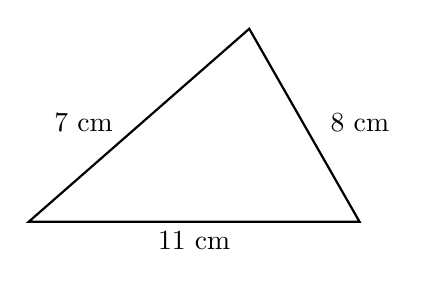
\begin{tikzpicture}[scale=0.7]
  \draw[thick] (0,0) -- (6,0) -- (4,3.5) -- cycle;
  \node[below] at (3,0) {$11$ cm};
  \node[left] at (1.7,1.8) {$7$ cm};
  \node[right] at (5.3,1.8) {$8$ cm};
\end{tikzpicture}
\end{center}
\end{questionText}
\correctAnswer{Yes, it satisfies the inequality and is unique}
\explanation{$7 + 8 = 15 > 11$ \checkmark, $7 + 11 = 18 > 8$ \checkmark, $8 + 11 = 19 > 7$ \checkmark. SSS with valid lengths produces exactly one unique triangle.}
\end{practiceQuestion}

\begin{practiceQuestion}{6-5-q24}{sa}
\begin{questionText}
Is it possible to get a circular cross-section from a rectangular prism? Explain.
\end{questionText}
\correctAnswer{No}
\explanation{A rectangular prism has only flat faces and straight edges. All cross-sections are polygons (triangles, rectangles, pentagons, hexagons). A circular cross-section requires a curved surface.}
\end{practiceQuestion}

\begin{practiceQuestion}{6-6-q19}{sa}
\begin{questionText}
Find the complement of $67°$.
\end{questionText}
\correctAnswer{$23°$}
\explanation{$90° - 67° = 23°$.}
\end{practiceQuestion}

\begin{practiceQuestion}{7-1-q13}{mc}
\begin{questionText}
A circle has a circumference of $31.4$ cm. Using $\pi \approx 3.14$, what is the diameter?
\end{questionText}
\choiceA{$5$ cm}
\choiceB{$10$ cm}
\choiceC{$15$ cm}
\choiceD{$20$ cm}
\correctAnswer{B}
\explanation{$d = C \div \pi = 31.4 \div 3.14 = 10$ cm.}
\end{practiceQuestion}

\begin{practiceQuestion}{7-5-q16}{mc}
\begin{questionText}
If all dimensions of a rectangular prism are doubled, what happens to its surface area?
\end{questionText}
\choiceA{It doubles}
\choiceB{It triples}
\choiceC{It quadruples}
\choiceD{It increases by a factor of $8$}
\correctAnswer{C}
\explanation{Surface area depends on the square of the dimensions. Doubling all dimensions multiplies each face area by $2^2 = 4$, so the total surface area quadruples.}
\end{practiceQuestion}

\begin{practiceQuestion}{7-6-q09}{mc}
\begin{questionText}
What unit is used to measure volume?
\end{questionText}
\choiceA{Square units (cm$^2$)}
\choiceB{Cubic units (cm$^3$)}
\choiceC{Linear units (cm)}
\choiceD{Degrees}
\correctAnswer{B}
\explanation{Volume measures three-dimensional space and is measured in cubic units.}
\end{practiceQuestion}

\begin{practiceQuestion}{7-7-q12}{mc}
\begin{questionText}
A cylindrical candle has a radius of $2$ cm and a height of $15$ cm. How much wax is needed to make the candle? Use $\pi \approx 3.14$.
\end{questionText}
\choiceA{$94.2$ cm$^3$}
\choiceB{$188.4$ cm$^3$}
\choiceC{$376.8$ cm$^3$}
\choiceD{$60$ cm$^3$}
\correctAnswer{B}
\explanation{$V = \pi r^2 h = 3.14 \times 4 \times 15 = 188.4$ cm$^3$.}
\end{practiceQuestion}

\begin{practiceQuestion}{8-1-q08}{mc}
\begin{questionText}
A sample of $40$ out of $2{,}000$ voters is surveyed. What fraction of the population is in the sample?
\end{questionText}
\choiceA{$\frac{1}{50}$}
\choiceB{$\frac{1}{40}$}
\choiceC{$\frac{1}{20}$}
\choiceD{$\frac{1}{500}$}
\correctAnswer{A}
\explanation{$\frac{40}{2{,}000} = \frac{1}{50}$.}
\end{practiceQuestion}

\begin{practiceQuestion}{8-3-q26}{gmc}
\begin{questionText}
The box plots below compare test scores for Class A and Class B.

\begin{center}
\begin{tikzpicture}[scale=0.1]
  \draw[thick,->] (49,0) -- (101,0);
  \foreach \x in {50,55,...,100} {
    \draw (\x,0.5) -- (\x,-0.5);
    \node[below,font=\small] at (\x,-0.5) {$\x$};
  }
  % Class A: min=60, Q1=70, med=78, Q3=85, max=95
  \draw[thick] (60,6) -- (95,6);
  \draw[thick,fill=funBlue!30] (70,4) rectangle (85,8);
  \draw[very thick,funBlue] (78,4) -- (78,8);
  \draw[thick] (60,4) -- (60,8);
  \draw[thick] (95,4) -- (95,8);
  \node[right,font=\small] at (96,6) {Class A};
  % Class B: min=50, Q1=58, med=65, Q3=72, max=80
  \draw[thick] (50,14) -- (80,14);
  \draw[thick,fill=funGreen!30] (58,12) rectangle (72,16);
  \draw[very thick,funGreen] (65,12) -- (65,16);
  \draw[thick] (50,12) -- (50,16);
  \draw[thick] (80,12) -- (80,16);
  \node[right,font=\small] at (81,14) {Class B};
\end{tikzpicture}
\end{center}

Which statement is best supported by the box plots?
\end{questionText}
\choiceA{Class B scored higher than Class A}
\choiceB{Class A has a higher median and a larger IQR}
\choiceC{Class A has a higher median and both classes have the same IQR}
\choiceD{Class A and Class B overlap, but Class A's median is higher}
\correctAnswer{D}
\explanation{Class A median $= 78$, Class B median $= 65$. Class A's range ($60$--$95$) overlaps with Class B's range ($50$--$80$), but Class A is higher overall.}
\end{practiceQuestion}

\begin{practiceQuestion}{8-4-q13}{mc}
\begin{questionText}
Store A daily sales: mean $\$500$, MAD $\$40$. Store B daily sales: mean $\$620$, MAD $\$40$. The difference in means in MADs is:
\end{questionText}
\choiceA{$1.5$ MADs}
\choiceB{$3$ MADs}
\choiceC{$40$ MADs}
\choiceD{$120$ MADs}
\correctAnswer{B}
\explanation{Difference $= \$620 - \$500 = \$120$. In MADs: $\frac{120}{40} = 3$ MADs.}
\end{practiceQuestion}

\begin{practiceQuestion}{8-5-q15}{mc}
\begin{questionText}
What is the mean of the data shown?

\begin{center}
\begin{tabular}{r|l}
\textbf{Stem} & \textbf{Leaf} \\
\hline
$1$ & $0\;\;5$ \\
$2$ & $0\;\;5$ \\
$3$ & $0$
\end{tabular}
\end{center}
\end{questionText}
\choiceA{$15$}
\choiceB{$18$}
\choiceC{$20$}
\choiceD{$25$}
\correctAnswer{C}
\explanation{Data: $10, 15, 20, 25, 30$. Mean $= \frac{10+15+20+25+30}{5} = \frac{100}{5} = 20$.}
\end{practiceQuestion}

\begin{practiceQuestion}{8-6-q19}{sa}
\begin{questionText}
A circle graph shows $35\%$ for music, $25\%$ for art, and the rest for drama. What percent is drama?
\end{questionText}
\correctAnswer{$40\%$}
\explanation{$100\% - 35\% - 25\% = 40\%$.}
\end{practiceQuestion}

\begin{practiceQuestion}{9-4-q30}{gsa}
\begin{questionText}
The table below shows a probability model for a game spinner. One probability is missing. Find the missing probability for outcome D.

\begin{center}
\begin{tabular}{|c|c|}
\hline
\textbf{Outcome} & \textbf{Probability} \\
\hline
A & $0.30$ \\
\hline
B & $0.25$ \\
\hline
C & $0.15$ \\
\hline
D & ? \\
\hline
\end{tabular}
\end{center}
\end{questionText}
\correctAnswer{$0.30$}
\explanation{$P(D) = 1 - (0.30 + 0.25 + 0.15) = 1 - 0.70 = 0.30$.}
\end{practiceQuestion}

\begin{practiceQuestion}{9-6-q06}{mc}
\begin{questionText}
Two dice are rolled. What is the probability that both dice show the same number (doubles)?
\end{questionText}
\choiceA{$\frac{1}{36}$}
\choiceB{$\frac{1}{12}$}
\choiceC{$\frac{1}{6}$}
\choiceD{$\frac{1}{3}$}
\correctAnswer{C}
\explanation{Doubles: $(1,1), (2,2), (3,3), (4,4), (5,5), (6,6)$ — that is $6$ out of $36$. $P = \frac{6}{36} = \frac{1}{6}$.}
\end{practiceQuestion}

\begin{practiceQuestion}{9-7-q25}{sa}
\begin{questionText}
A student runs $200$ simulation trials for an event with theoretical probability $\frac{1}{4}$. They observe the event $54$ times. What is the experimental probability? Is it close to the theoretical value?
\end{questionText}
\correctAnswer{$0.27$; yes, it is close to $0.25$}
\explanation{$P = \frac{54}{200} = 0.27$. Theoretical $= 0.25$. The difference of $0.02$ is small, especially with $200$ trials.}
\end{practiceQuestion}
